\documentclass[12pt]{article}
\usepackage[margin=1in]{geometry}% Change the margins here if you wish.
\setlength{\parindent}{0pt} % This is the set the indent length for new paragraphs, change if you want.
\setlength{\parskip}{5pt} % This sets the distance between paragraphs, which will be used anytime you have a blank line in your LaTeX code.
\pagenumbering{gobble}% This means the page will not be numbered. You can comment it out if you like page numbers.

%------------------------------------

% These packages allow the most of the common "mathly things"
\usepackage{amsmath,amsthm,amssymb}
\usepackage{sectsty}

% This package allows you to add images.
\usepackage{graphicx, tikz-cd, adjustbox}
\usepackage{float}
\usepackage{scalerel}
\usepackage{stackengine,wasysym}
\usepackage{biblatex}
\addbibresource{biblio.bib}

\newcommand\reallywidetilde[1]{\ThisStyle{%
  \setbox0=\hbox{$\SavedStyle#1$}%
  \stackengine{-.1\LMpt}{$\SavedStyle#1$}{%
    \stretchto{\scaleto{\SavedStyle\mkern.2mu\AC}{.5150\wd0}}{.6\ht0}%
  }{O}{c}{F}{T}{S}%
}}

% These are theorem environments.  This should cover everything you need, and you should be able to tell what environment goes with what type of result, but please let me know if I've missed anything.
\newtheoremstyle{mytheoremstyle} % name
    {\topsep}                    % Space above
    {\topsep}                    % Space below
    {}                   % Body font
    {}                           % Indent amount
    {\bf}                   % Theorem head font
    {.}                          % Punctuation after theorem head
    {.5em}                       % Space after theorem head
    {}  % Theorem head spec (can be left empty, meaning ‘normal’)

\theoremstyle{mytheoremstyle}

\newtheorem{proposition}{Proposition}[section]
\newtheorem{example}{Example}
\newtheorem{classtheorem}{Theorem}
\newtheorem{theorem}{Theorem}[section]
\newtheorem{challenge}[theorem]{Challenge}
\newtheorem{question}[theorem]{Question}
\newtheorem{problem}[theorem]{Problem}
\sectionfont{\fontsize{14}{15}\selectfont}
\subsectionfont{\fontsize{12}{15}\selectfont}

\newcommand{\bP}{\mathbb{P}}
\newcommand{\bA}{\mathbb{A}}
\newcommand{\bZ}{\mathbb{Z}}
\newcommand{\bC}{\mathbb{C}}
\newcommand{\bQ}{\mathbb{Q}}
\newcommand{\cO}{\mathcal{O}}
\newcommand{\cF}{\mathcal{F}}
\newcommand{\cM}{\mathcal{M}}
\newcommand{\ds}{\displaystyle}
\newcommand{\al}{\alpha}
\newcommand{\li}{l^{\infty}}
\newcommand{\ep}{\varepsilon}
\newcommand{\de}{\delta}
\newcommand{\spec}{\text{Spec\hspace*{.5mm}}}
\newcommand{\mspec}{\text{mSpec\hspace*{.5mm}}}
\newcommand{\tor}{\text{Tor}}
\newcommand{\cS}{\mathcal{S}}
\newcommand{\cR}{\mathcal{R}}
\newcommand{\cN}{\mathcal{N}}
 
%These help to format the names of the results the way we are in class and in notes.
%\renewcommand*{\proposition}{\Roman{section}.\arabic{theorem}}
\renewcommand*{\thetheorem}{\arabic{section}.\arabic{theorem}}
\renewcommand*{\theclasstheorem}{\Alph{theorem}}
\renewcommand*{\thechallenge}{\arabic{section}.\arabic{theorem}}
\renewcommand*{\thequestion}{\arabic{section}.\arabic{theorem}}
\renewcommand*{\theproblem}{\arabic{section}.\arabic{theorem}}
% Put the name of your paper here. It does not need to be a fancy name, but should tell the reader what is contained in the paper.
\title{Flat Modules}

% You are the author, put your name here.
\author{Nutan Nepal}

% You can change the date to be something other than the current date if you want.
\date{\today}

\begin{document}
\maketitle

\makebox[\linewidth]{\rule{200mm}{1pt}}
\section{Introduction}
\hspace*{8mm}In the study algebraic sets, we can consider a family of varieties as
follows: using the coordinate ring $R$ of an
affine variety $Y$ over an algebraically closed field $k$ and a collection
of polynomials $f_i(x_1,\ldots,x_n; b)\in R[x_1,\ldots,x_n]$, we consider
the collection of zero sets
$$V(f_i(x;b))=\{a\in \mathbb{A}^n_k\mid \ f_i(a,b)=0\},\ \ \ b\in Y$$ to be
in \textbf{a family parametrized by $Y$}. The fibers over each $b\in Y$
have covering by affine varieties and can be considered
as subschemes of $\bA^n_k$.
If $I$ is the ideal generated by the polynomials $f_i$'s
in the ring $R[x_1,\ldots,x_n]$,
then we get the ring morphism $f\colon R\to R[x_1,\ldots,x_n]/I$.
This ring morphism induces the morphism of the maximal spectrums (the topological
space with maximal ideals as the points)
$$\mspec (R[x_1,\ldots,x_n]/I) \to \mspec R = Y$$
which describes the maps between the subschemes $V(I)$ and $Y$.
The fiber over each point $b\in Y$ is then given by
$$\mspec (R[x_1,\ldots,x_n]/I\otimes R/m_b)=\mspec (k[x_1,\ldots,x_n]
    /(f_i(x,b))).$$
The well-behavedness of the fibers over Y depends on the family of
the subschemes i.e. on the morphisms of the subschemes.
\begin{example}
    The projection
    $$\{(x,y,t)\in \bA^3_k\mid y-xt=0\}\to \bA^2_k$$
    defines a family of subvarieties of the $V(y-xt)$.
    The morphism has fiber over $(0,0)$ as one-dimensional variety
    (since any value of $t$
    satisfies the polynomial) and the fibers over other points are
    zero-dimensional.$\blacktriangle$
\end{example}

\begin{figure}
    \label{fig:M1}
    \centering{
        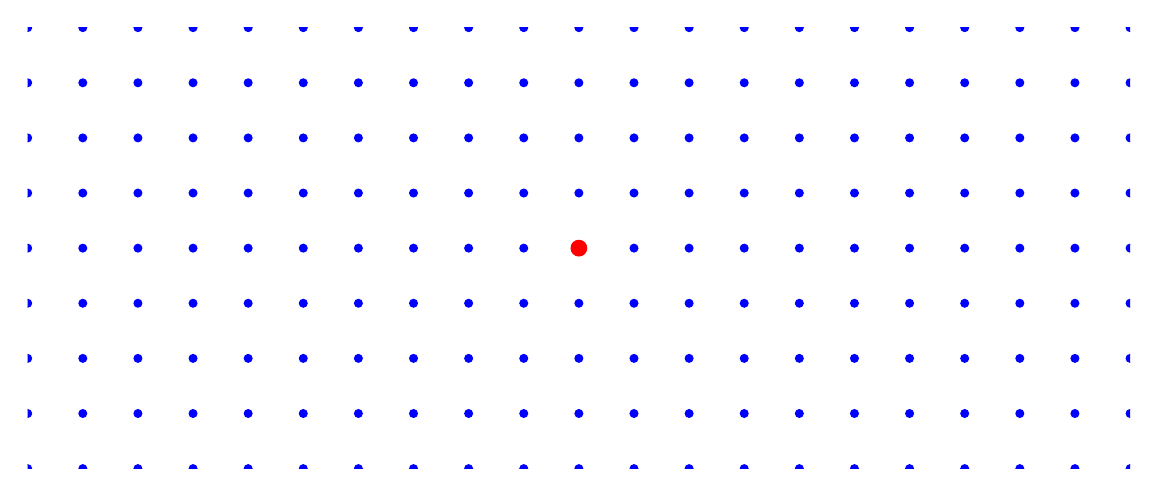
\begin{tikzpicture}[scale=.7]
            \begin{scope}

                \clip (20,0) rectangle (40,8); % Clips the picture...
                %\draw[red, thick] (30,0) -- (30,10);
                %\pgftransformcm{1.4}{0}{2}{0.8}{\pgfpoint{0cm}{0cm}} % This is actually the transformation
                %  matrix entries that gives the slanted
                % unit vectors. You might check it on
                % MATLAB etc. . I got it by guessing.
                \foreach \x in {0,1,...,40}{                           % Two indices running over each
                        \foreach \y in {0,1,...,40}{                       % node on the grid we have drawn 
                                \node[draw,circle,inner sep=1pt,fill, color=blue] at (\x,\y) {}; % Places a dot at those points
                            }
                    }
                \node[draw,circle,inner sep=2pt,fill, color=red] at (30,4) {};
                %\draw[style=help lines,thin] (0,0) grid[step=1cm] (40,40);
            \end{scope}
        \end{tikzpicture}
    }
    \caption{Fibers over integer lattice points are shown in the diagram. The blue points are the zero dimensional fibers and the red
        is the line (one-dimensional fiber) over the point (0,0).}
\end{figure}

\hspace*{8mm}Hence, a morphism of varieties $f\colon X\to Y$ itself defines a family of subvarieties
of the source parametrized by the target. The families where the
fibers vary ``nicely'' are called \textbf{flat families} and these
families are characterized by \textbf{flat morphisms} between
the subschemes. In the above example, the fibers of projection had
jumps in their dimensions.
The notion of flatness was first introduced by
Serre for algebraic reasons and Grothendieck later recognized the
geometric significance of it.\cite{vakil2023foundations}

\vspace*{2mm}
\hspace*{8mm}Similar considerations with homogenous polynomials
in $R[x_0,\ldots,x_n]$
defines a family of subschemes of $\bP^n_k$.
Here we describe the notion of flat morphisms
between two schemes.

\section{Flat modules and flat maps}

\hspace*{8mm}For any $A$-module $M$, every short exact sequence
$0\longrightarrow N'\longrightarrow N\longrightarrow N''
    \longrightarrow 0$ of $A-$ modules induces the exact sequence
$ N'\otimes M\longrightarrow N\otimes M
    \longrightarrow N''\otimes M\longrightarrow 0$.
An $A$-module $M$ is flat if for every short exact sequence
$\mathcal{S}:$
$0\longrightarrow N'\longrightarrow N\longrightarrow N''
    \longrightarrow 0$, the induced sequence $\mathcal{S}\otimes M:$
$$0\longrightarrow N'\otimes M\longrightarrow N\otimes M
    \longrightarrow N''\otimes M\longrightarrow 0$$
is also exact. $M$ is called faithfully flat if we have:
$\mathcal{S}\text{ exact}\iff \mathcal{S}\otimes M \text{ exact}.$
A ring homomorphism $f\colon R \to S$ is called flat (resp. faithfully flat)
if $S$ is flat (resp. faithfully flat) as
an $R$-module.

\begin{example}
    $\blacktriangle$
\end{example}


While the definition looks quite unmotivating,
the following list provides plenty of examples and general
facts about flat modules.

\subsection*{Examples and facts:}
\begin{enumerate}
    \item Projective modules are flat. Injective modules need not be flat
          and flat modules need not be projective or injective. In particular,
          free modules are flat.
    \item $\mathbb{Z}$ is a projective (and hence, flat) $\bZ$-module.
          In general, $-\otimes_A A$ is the identity endofunctor in
          the category of $A$-modules
          i.e. $\cS\otimes_A A = \cS$ and so,
          $A$ is always a flat $A$-module.
    \item $\bQ$ is a flat $\bZ$-module. ($\bQ$ is also an injective
          $\bZ$-module)
    \item Flat modules are torsion-free. Hence, the $\bZ$-modules
          $\bZ/n\bZ$ and $\bQ/\bZ$ are not flat. The latter is an example
          of injective module that is not flat.
    \item Finitely generated modules over principal ideal domains are
          flat if and only if they are torsion-free if and only if they
          are free.
    \item The direct sum of flat modules are flat (since the tensor
          product commutes with arbitrary direct sums). In particular,
          the $\bZ$-module $\bQ\oplus\bZ$ (which is neither projective
          nor injective) is flat.
    \item The localization $S^{-1}N$ of an $A$-module $N$ by the multiplicative
          set $S$ of $A$ is an exact functor. So $A\to S^{-1}A$ is a flat ring
          morphism.
    \item Flatness is preserved by change of base ring:
          If $M$ is a flat $B$-module and $B\to A$ is a ring morphism,
          then $M\otimes_B A$ is a flat $A$-module.
    \item Flatness is preserved by composition:
          If $A$ is a flat $B$-algebra and $M$ is a flat $A$-module, then
          $M$ is also $B-$flat.
    \item Flatness is a local property:
          An $A$-module $M$ is $A$-flat if and only if $M_\mathfrak{p}$
          is $A_\mathfrak{p}$-flat for all prime ideals $\mathfrak{p}
              \subset A$.
    \item An $A$-module $M$ is $A$-flat if and only if for all ideals $I$
          of $A$, we have $I\otimes M\cong IM$.
\end{enumerate}

\section{Quasicoherent sheaves and flat morphisms}
\hspace*{8mm}Given a ring $A$ and an
$A$-module $M$, we can form a sheaf of abelian
groups $\widetilde{M}$ on $X= \spec R$ by taking $\widetilde{M}(D(f))
    = M\otimes f^{-1}A = f^{-1}M$, which is the localization of $M$ by the
multiplicative set $\{1,f,f^2,\ldots\}$, and then extending to
all the open sets. The sheaf $\widetilde{M}$
has the structure of an $\cO_X$-module: each $\widetilde{M}(U)$ is
an $A(U)$-module and the module action commutes with the restriction maps.
In other words, the following diagram commutes:

\vspace*{3mm}
\adjustbox{scale=0.7,center}{%
    \begin{tikzcd}
        {\mathcal{O}_X(V)\times\mathcal{F}(V)} &&& {\mathcal{F}(V)} \\
        \\
        \\
        {\mathcal{O}_X(U)\times\mathcal{F}(U)} &&& {\mathcal{F}(U)}
        \arrow["{\text{res}_{V,U}\times\text{res}_{V,U}}"', from=1-1, to=4-1]
        \arrow["action", from=1-1, to=1-4]
        \arrow["{\text{res}_{V,U}}"', from=1-4, to=4-4]
        \arrow["action", from=4-1, to=4-4]
    \end{tikzcd}
}

\begin{enumerate}

    \item A sheaf $\cF$ on $X$ is called \textbf{quasicoherent} if for each affine
          open subset Spec $A$ of $X$, the sheaf $\cF|_{\spec A}$
          is isomorphic to $\widetilde{M}$ for some $A$-module $M$.
          The category of quasicoherent sheaves over an affine
          scheme $\spec A$ is equivalent to the category of $A$-modules:
          $\mathcal{QC}oh_{\spec A} \tilde{\longleftrightarrow}
              \mathfrak{mod}_A$.

    \item A \textbf{quasicoherent sheaf} $\cF$ on $X$ is said to be
          \textbf{flat} at $p\in X$
          if $\cF_p$ is a flat $\cO_{X,p}$-module.
          A \textbf{quasicoherent sheaf} $\cF$ on $X$ is said to be
          \textbf{flat} over $X$
          if for every point $p\in X$, $\cF_p$ is a flat
          $\cO_{X,p}$-module.

    \item A morphism $f\colon X\to Y$ of schemes is said to be \textbf{flat}
          at $p\in X$ if $\cO_{X,p}$ is a flat
          $\cO_{Y,f(p)}$-module.
          A morphism $f\colon X\to Y$ of schemes is called a \textbf{flat
              morphism} if for every $p\in X$, $\cO_{X,p}$ is a flat
          $\cO_{Y,f(p)}$-module.
          A morphism is called \textbf{faithfully flat} if it is both
          flat and surjective.

          In particular, if $Y=\mspec A$, a morphism (or family)
          of schemes
          $f\colon X\to Y$ is flat if $\cO(U)$ is a flat $A$-module for every
          open set $U\subset X$.

\end{enumerate}

\subsection*{Examples and facts}
\begin{enumerate}
    \item Given a ring map $B\to A$, $A$ is faithfully flat over $B$
          if and only if $\spec A\to\spec B$ is a faithfully flat morphism.
    \item Open embeddings are flat. $f\colon X\to Y$ is an \textbf{open
              embedding} if $X$ is isomorphic to an open set of $Y$. For a
          morphism $f\colon D(y-x^2)\to \bA^2_k$ which is clearly an open
          embedding we see that
    \item A morphism of rings $A\to B$ is flat if and only if the
          corresponding morphism of schemes $\spec B\to\spec A$.
          More generally, if $B\to A$ is a ring homomorphism and $M$ is
          an $A$-module, then $M$ is $B-$flat if and only if
          $\widetilde{M}$ is flat over $\spec B$.
    \item The fibers of a flat morphism of varieties $f\colon X\to Y$ all
          all have the same dimension dim $X-$ dim $Y$.
    \item If $f\colon X\to Y$ is a surjective morphism of a variety to
          a non-singular curve, then it is flat.
    \item The above two statements imply: The fibers of a surjective
          morphism of a variety to a non-singular curve have dimension
          equal to dim $X-1$.
\end{enumerate}

\section{Flatness through $\tor$}
\hspace*{8mm}$\tor^A_i(M,\cdot)$ is the derived functor
$\mathfrak{mod}_A\to\mathfrak{mod}_A$
of the right-exact covariant functor
$M\otimes\cdot$ (meaning $\tor^A_0(M,N)
    =M\otimes N$ for all $A$-modules $N$).
For an $A$-module $M$, the following are equivalent:
\begin{enumerate}
    \item[i.] $M$ is a flat $A-$ module.
    \item[ii.] $\tor^A_i(M,N)=0$ for all $i>0$ and $A$-module N.
    \item[iii.] $\tor^A_1(M,N)=0$ for all $A$-module N.
\end{enumerate}

Tor stands for torsion as seen in the following example:
\begin{example}
    If $x\in A$ is not a zero divisor then
    $$\tor^A_i(M,A/(x))=\begin{cases}
            M/xM  & \text{if } i=0; \\
            (M:x) & \text{if } i=1; \\
            0     & \text{if } i>1,
        \end{cases}$$
    where $(M:x)=\{m\in M\mid x\cdot m=0\}$ is the set of elements
    annihilated by $x$. Hence a module over a domain is flat if and
    only if it is torsion-free.$\blacktriangle$
\end{example}

\subsection{Examples and facts}
\begin{enumerate}
    \item (\textbf{ideal-theoretic criterion for flatness}) An
          $A$-module $M$ is flat if and only if $\tor^A_1(M,A/I)=0$
          for any ideal $I$.
\end{enumerate}

\section{}
\hspace*{8mm} A lot of the nice properties that we find in flat morphism
turn out to be cohomological in nature. This makes sense since flatness itself
is characterized by cohomology: it is equivalent to the vanishing of the Tor
functor. For example, if $f\colon X\to Y$ is a projective flat morphism with
$Y$ connected and Noetherian, then the numerical invariants of the fibers like
the dimension, Hilbert polynomial, degree, the arithmetic genus and other numbers
interpretable in terms of an Euler characteristic are constant \cite{vakil2023foundations}.

\newpage

\setcounter{section}{1}
\setcounter{theorem}{1}

\printbibliography
\end{document}